\newpage
\section*{A: Tien Phong warehouse situation}
    \phantomsection\addcontentsline{toc}{subsection}{\numberline {}A. Tien Phong warehouse situation}
    \label{apx:A}

\subsection*{A.1. Layout and design}

    \begin{figure}[!ht]
        \centering
        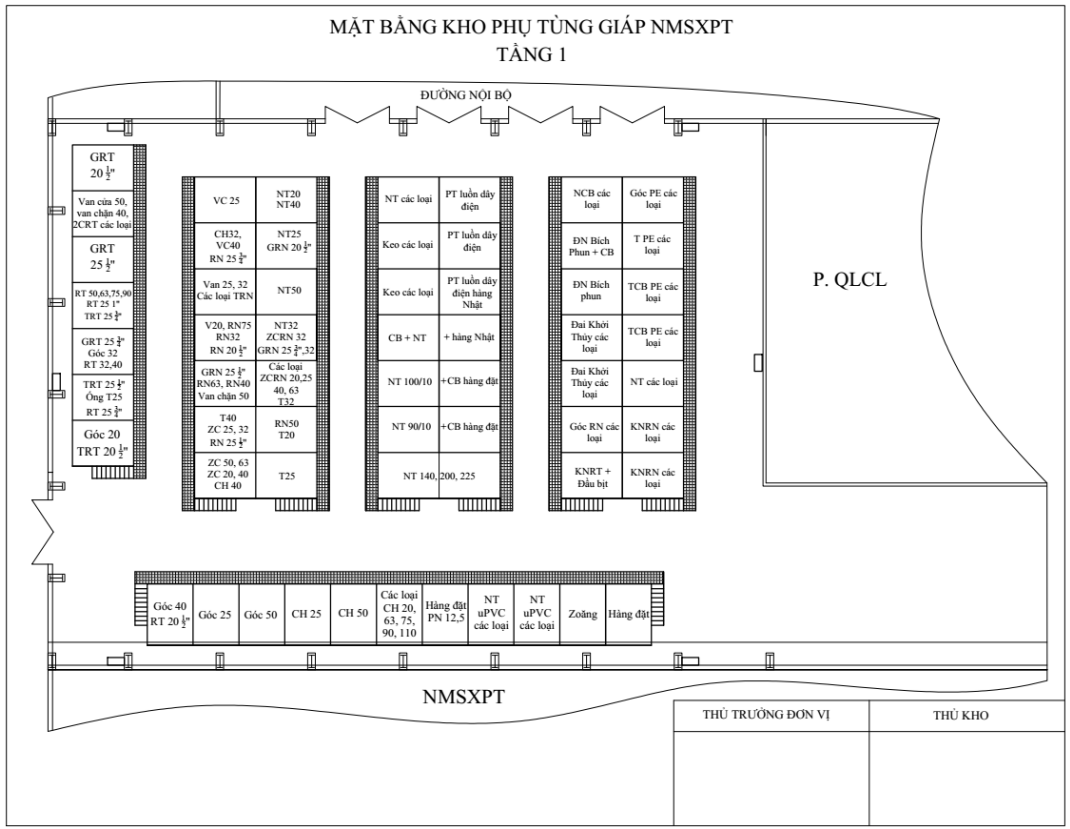
\includegraphics[scale=0.7]{figure/premises.png}
        \caption{Warehouse premises}
        \label{fig:premiese}
    \end{figure}

    \begin{figure}[!ht]
        \centering
        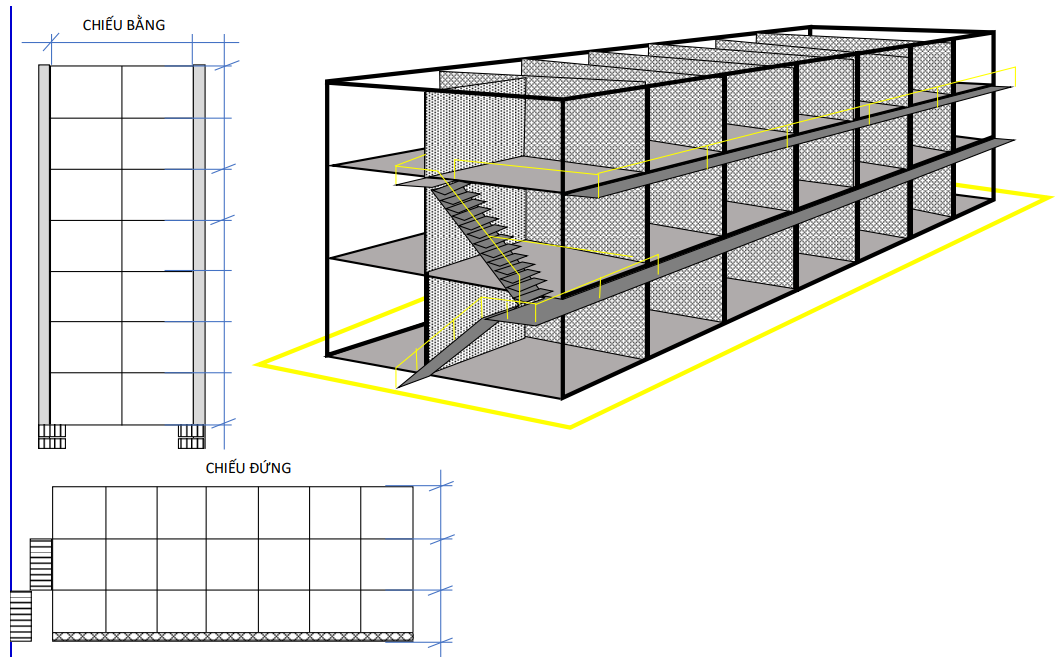
\includegraphics[scale=0.55]{figure/design.png}
        \caption{Warehouse design}
        \label{fig:design}
    \end{figure}
    
    \begin{table}[]
        \centering
        \caption{Storage capacity}
        \begin{tabularx}{1\textwidth}{
            | >{\centering\arraybackslash}y
            | >{\centering\arraybackslash}y
            | >{\centering\arraybackslash}y
            | >{\centering\arraybackslash}y
            | >{\centering\arraybackslash}y
            | >{\centering\arraybackslash}y
            |
            }
            \hline 
            \bfseries Type  
            &\bfseries Location per floor  
            &\bfseries Number of floors
            &\bfseries Number of locations
            &\bfseries Capacity \linebreak ${(m^3)}$
            \\\hline Single 7 & 7 & 3 & 21 & 504 
            \\\hline Single 11 & 11 & 3 & 33 & 792 
            \\\hline Double & 14 & 3 & 42 & 1008
            \\\hline
        \end{tabularx}
        \label{tab:storagecapacity}
    \end{table}

\subsection*{A.2. Management processes}

    \begin{figure}[!ht]
        \centering
        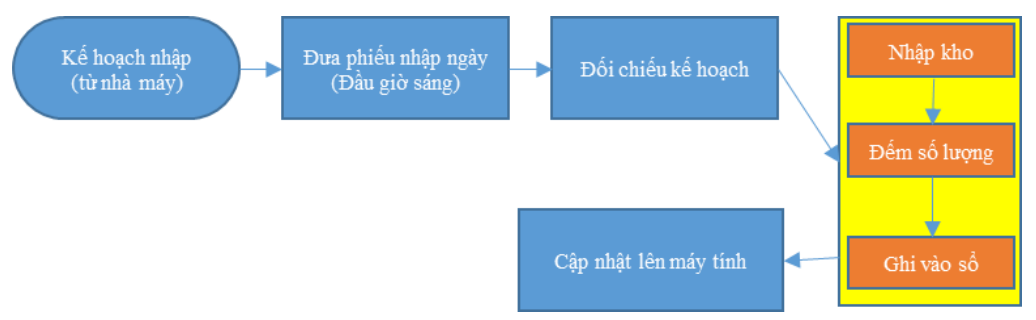
\includegraphics[scale=0.5]{figure/receiveproc.png}
        \caption{Current receiving and put-away process}
        \label{fig:currentrap}
    \end{figure}
    
    \begin{figure}[!ht]
        \centering
        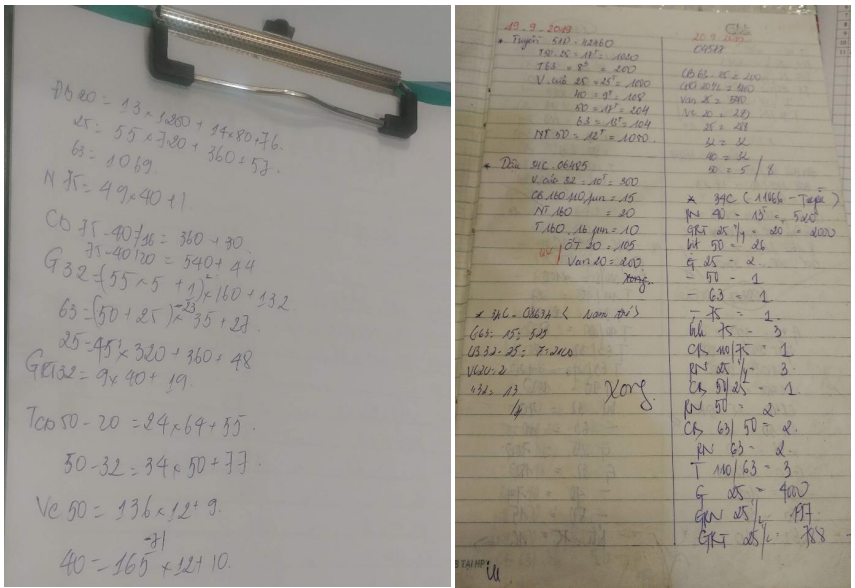
\includegraphics[scale=0.5]{figure/handcounting.png}
        \caption{Manual labour counting}
        \label{fig:manuallabour}
    \end{figure}
    
    \begin{figure}[!ht]
        \centering
        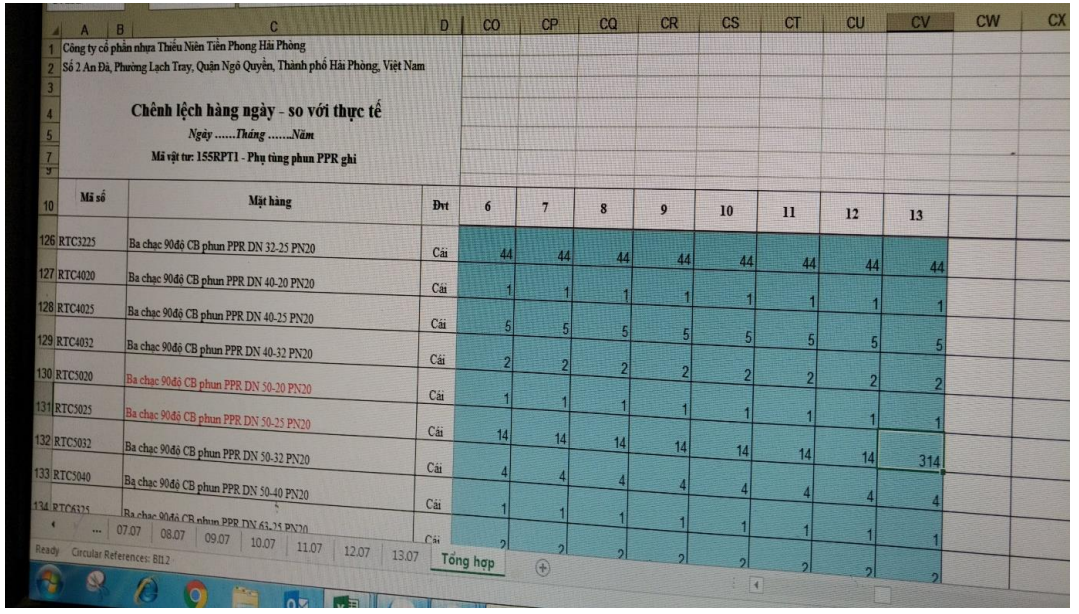
\includegraphics[scale=0.4]{figure/excel.png}
        \caption{Current way to record information}
        \label{fig:recinf}
    \end{figure}
    
    \begin{figure}[!ht]
        \centering
        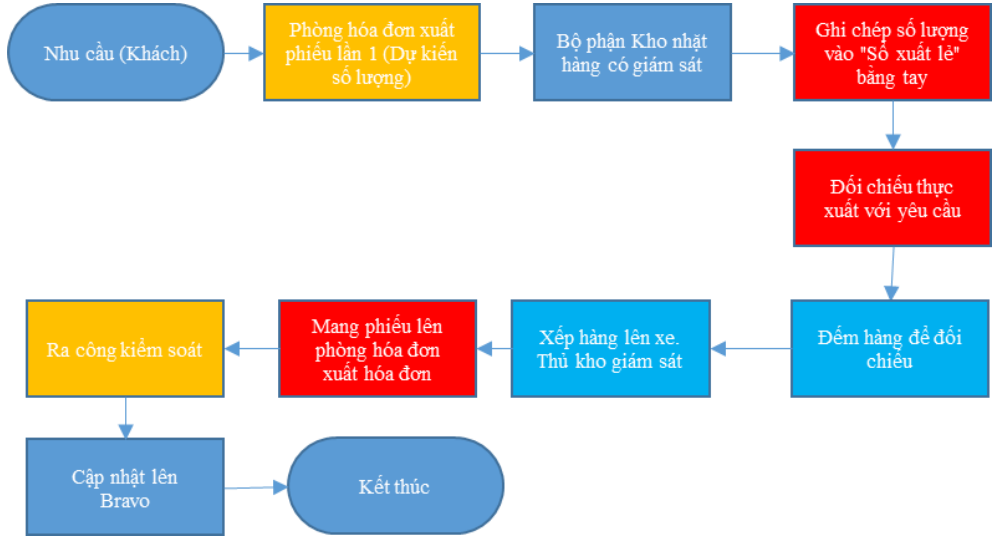
\includegraphics[scale=0.5]{figure/orderproc.png}
        \caption{Current order fulfillment process}
        \label{fig:currentof}
    \end{figure}
            
    \begin{figure}[!ht]
        \centering
        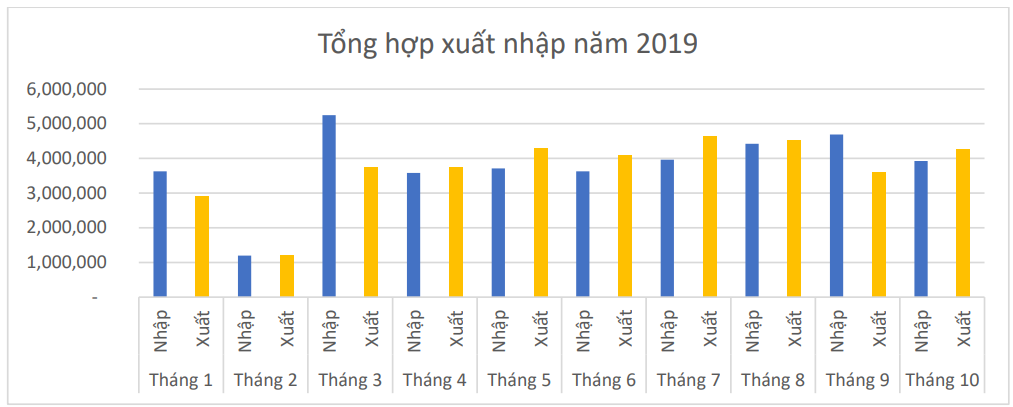
\includegraphics[scale=0.7]{figure/2019stas.png}
        \caption{Import and export report of 4 sections in 2019}
        \label{fig:rep2019}
    \end{figure}

Report shows that in the PP-R sections, the total amounts of imported and exported products (total products number is 434) are 37,991,108 and 36,982,276, respectively. The price range of PP-R products varies from a few thousand to several million VND for one product.